\documentclass{standalone}
\usepackage{tikz}
\usepackage{ctex,siunitx}
\setCJKmainfont{Noto Serif CJK SC}
\usepackage{tkz-euclide}
\usepackage{amsmath}
\usetikzlibrary{patterns, calc,3d}
\usetikzlibrary {decorations.pathmorphing,decorations.pathreplacing,decorations.shapes}
\tikzset{label style/.append style={font=\small}}
\begin{document}
\small
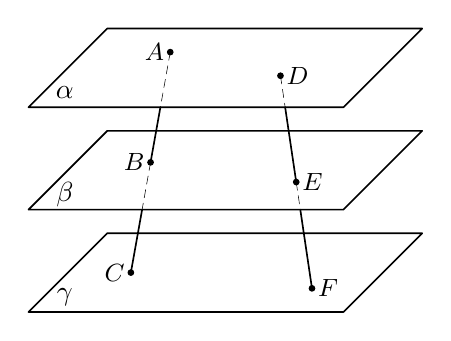
\begin{tikzpicture}[>=latex,scale=1.0,inner sep=2pt]
  \tkzDefPoints{0/0/M,4/0/N,5/1/P,1/1/Q,0/1.3/M',0/2.6/M'',1.8/3.3/A,1.3/0.5/C,3.2/3.0/D,3.6/0.3/F}
  \tkzDefPointsBy[translation=from M to M'](N,P,Q){N',P',Q'}
  \tkzDefPointsBy[translation=from M to M''](N,P,Q){N'',P'',Q''}
  \tkzDrawPolygon[semithick](M,N,P,Q)
  \tkzDrawPolygon[semithick](M',N',P',Q')
  \tkzDrawPolygon[semithick](M'',N'',P'',Q'')
  \tkzDefMidPoint(A,C)\tkzGetPoint{B}
  \tkzDefMidPoint(D,F)\tkzGetPoint{E}
  \tkzInterLL(A,B)(M'',N'')\tkzGetPoint{G}
  \tkzInterLL(B,C)(M',N')\tkzGetPoint{H}
  \tkzInterLL(D,E)(M'',N'')\tkzGetPoint{I}
  \tkzInterLL(E,F)(M',N')\tkzGetPoint{J}
  \tkzDrawPoints[fill=black](A,B,C,D,E,F)

  \tkzDrawSegments[semithick](B,G H,C E,I F,J)
  \tkzDrawSegments[densely dashed](A,G B,H D,I E,J)
  \tkzLabelAngle[pos=0.5](N',M',Q'){$\beta$}
  \tkzLabelAngle[pos=0.5](N,M,Q){$\gamma$}
  \tkzLabelAngle[pos=0.5](N'',M'',Q''){$\alpha$}
  \tkzLabelPoints[left](A,B,C)
  \tkzLabelPoints[right](D,E,F)
\end{tikzpicture}
\end{document}